\chapter{Aplicando IDRs e Outliers no GeoGuide}
\label{chap:aplicando}

% <TODO> [DEPRECATED]: "Esse capítulo ainda está bem inconsistente. É necessário analisar qual o real foco dele. Se ele não é um capítulo de experimentos, mas sim de uso, seria interessante vários prints do sistema para explicar o real uso desses conceitos."

Neste capítulo iremos mostrar como utilizamos os conceitos de IDRs e a abordagem de detecção de outliers no GeoGuide. Mostraremos o passo a passo de como utilizar a plataforma do GeoGuide, desde o passo da autenticação, passando pelo processo \textit{upload} de um dataset no formato \textit{csv}, mostrando como o GeoGuide trata esse conjunto de dados e então exemplificando a criação de IDRs na plataforma e a abordagem de detecção de outliers nesse conjunto.

\section{Carregando um dataset}

O primeiro passo para começar a utilizar o GeoGuide é realizar um cadastro básico do usuário (informando os campos \textit{e-mail}, \textit{senha} e \textit{confirmação de senha}) que está acessando a plataforma (ver Figura \ref{fig:geoguide-register}). Caso o usuário já possua conta na plataforma, então ele só precisará informar seu email e senha que usou durante o cadastro para poder ter acesso ao GeoGuide (ver Figura \ref{fig:geoguide-login}).

\begin{figure*}[h]
	\centering
	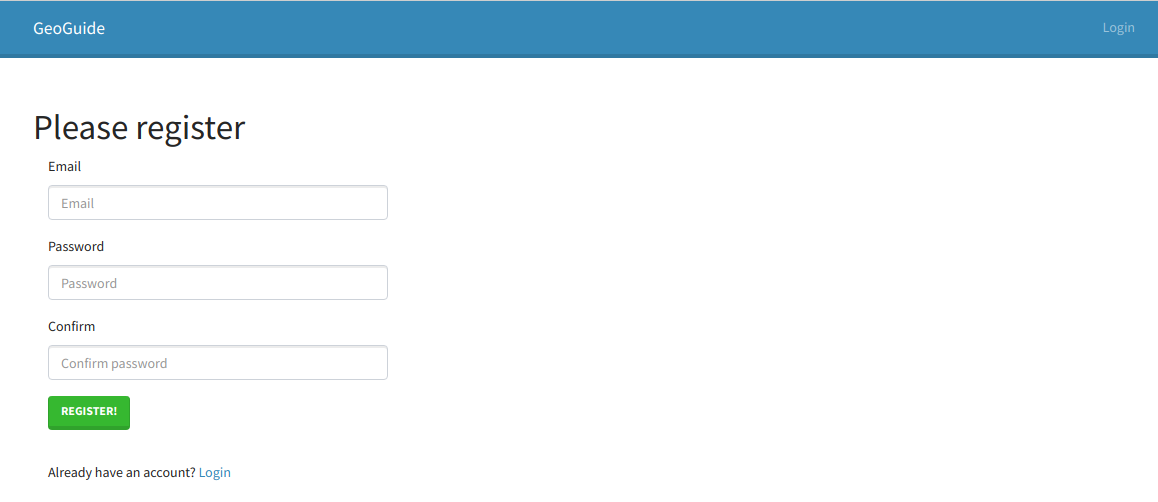
\includegraphics[width=\textwidth]{images/geoguide-register.png}
	\caption{Tela de registro de usuário do GeoGuide}
	\label{fig:geoguide-register}
	\vspace{-10pt}
\end{figure*}

Esse cadastro é importante para que o usuário possa registrar os datasets carregados e não precisar ficar fazendo o mesmo carregamento desses dados várias vezes, pois todas as suas configurações vão ficar registradas na plataforma e ligadas diretamente à sua conta de usuário.

\begin{figure*}[h]
	\centering
	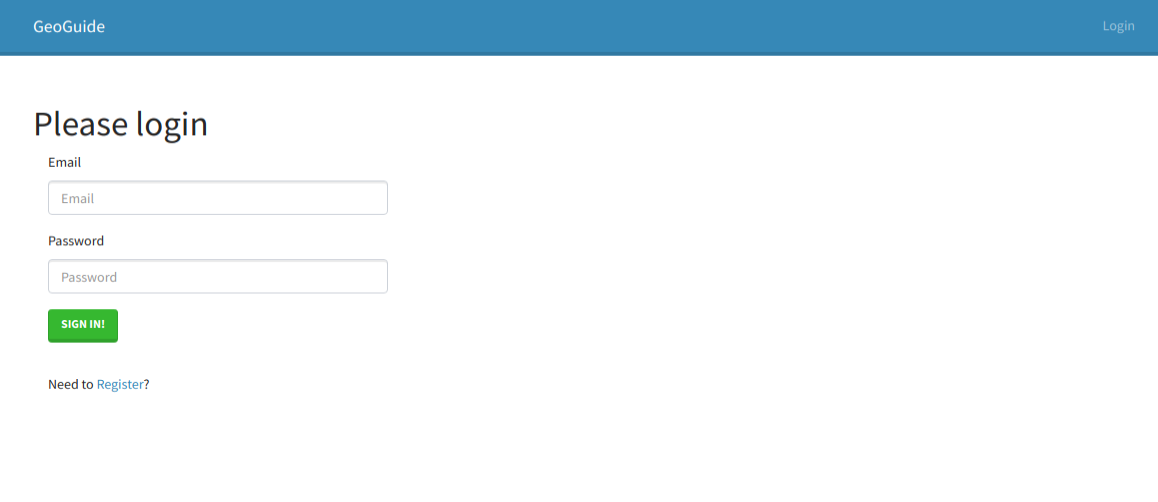
\includegraphics[width=\textwidth]{images/geoguide-login.png}
	\caption{Tela de login do usuário do GeoGuide}
	\label{fig:geoguide-login}
	\vspace{-10pt}
\end{figure*}

Após escolher qual conjunto de dados ele vai querer trabalhar, é preciso que ele realize o processo de carregamento de um arquivo .csv e então informar alguns dados básicos sobre aquele conjunto que vai estar registrando na sua conta, como por exemplo: qual o nome que ele vai atribuir àquele conjunto, quantas linhas do .csv vai levar em consideração no carregamento (isso é importante para caso o usuário deseje analisar somente uma parte do dataset), quais os campos que ele quer levar em consideração para o cálculo das métricas de \textit{similaridade} \textit{diversidade} e entre outras informações.

\begin{figure*}[h]
	\centering
	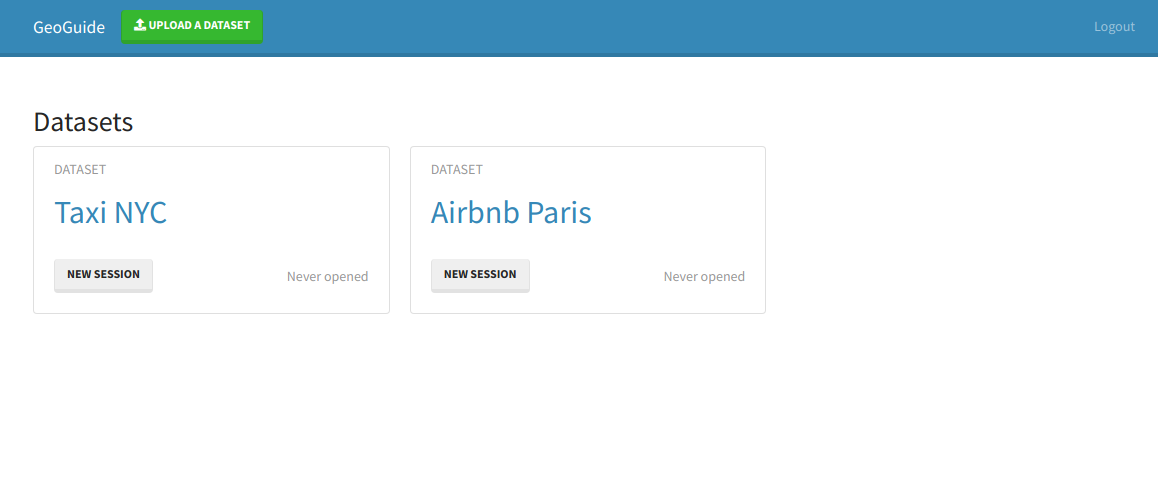
\includegraphics[width=\textwidth]{images/geoguide-datasets.png}
	\caption{Tela de datasets do usuário no GeoGuide}
	\label{fig:geoguide-datasets}
	\vspace{-10pt}
\end{figure*}

Quando finalizar o preenchimento do formulário referente ao dataset, então o analista poderá visualizar quais os datasets que já estão registrados na sua conta e selecionar qual ele irá querer trabalhar no momento. Após isso, o GeoGuide passará para o próximo passo que é a visualização desses dados espaciais num mapa global centralizado na localização do dataset, de forma que o usuário já possa interagir com os pontos no mapa, podendo realizar algumas filtragens e também clicando em cada ponto específico para mostrar seus atributos referentes ao seu domínio específico.

\section{Pré-processamento do GeoGuide}

Logo após o primeiro instante de plotagem do mapa global na tela do usuário, o servidor da plataforma do GeoGuide inicia, em paralelo e sem a intervenção do usuário, um processo para o cálculo das métricas de similaridade e diversidade de todos os pares de pontos possíveis no dataset.

Primeiro a ferramenta seleciona um ponto $a$ do dataset espacial e o compara com um ponto $b$ sendo seu sucessor no conjunto. A comparação leva em consideração os atributos ``não espaciais'' dos pontos e tem como resultado a métrica de \textit{similaridade} entre esses dois pontos. Então, é realizado uma segunda comparação para gerar a métrica de \textit{diversidade} entre os pontos. Para essa métrica, é levado em consideração os atributos geográficos desses pontos (\textit{latitude} e \textit{longitude}), de forma que, quanto mais distante um ponto $a$ é do ponto $b$, mais diverso eles serão.  

\begin{figure*}[h]
	\centering
	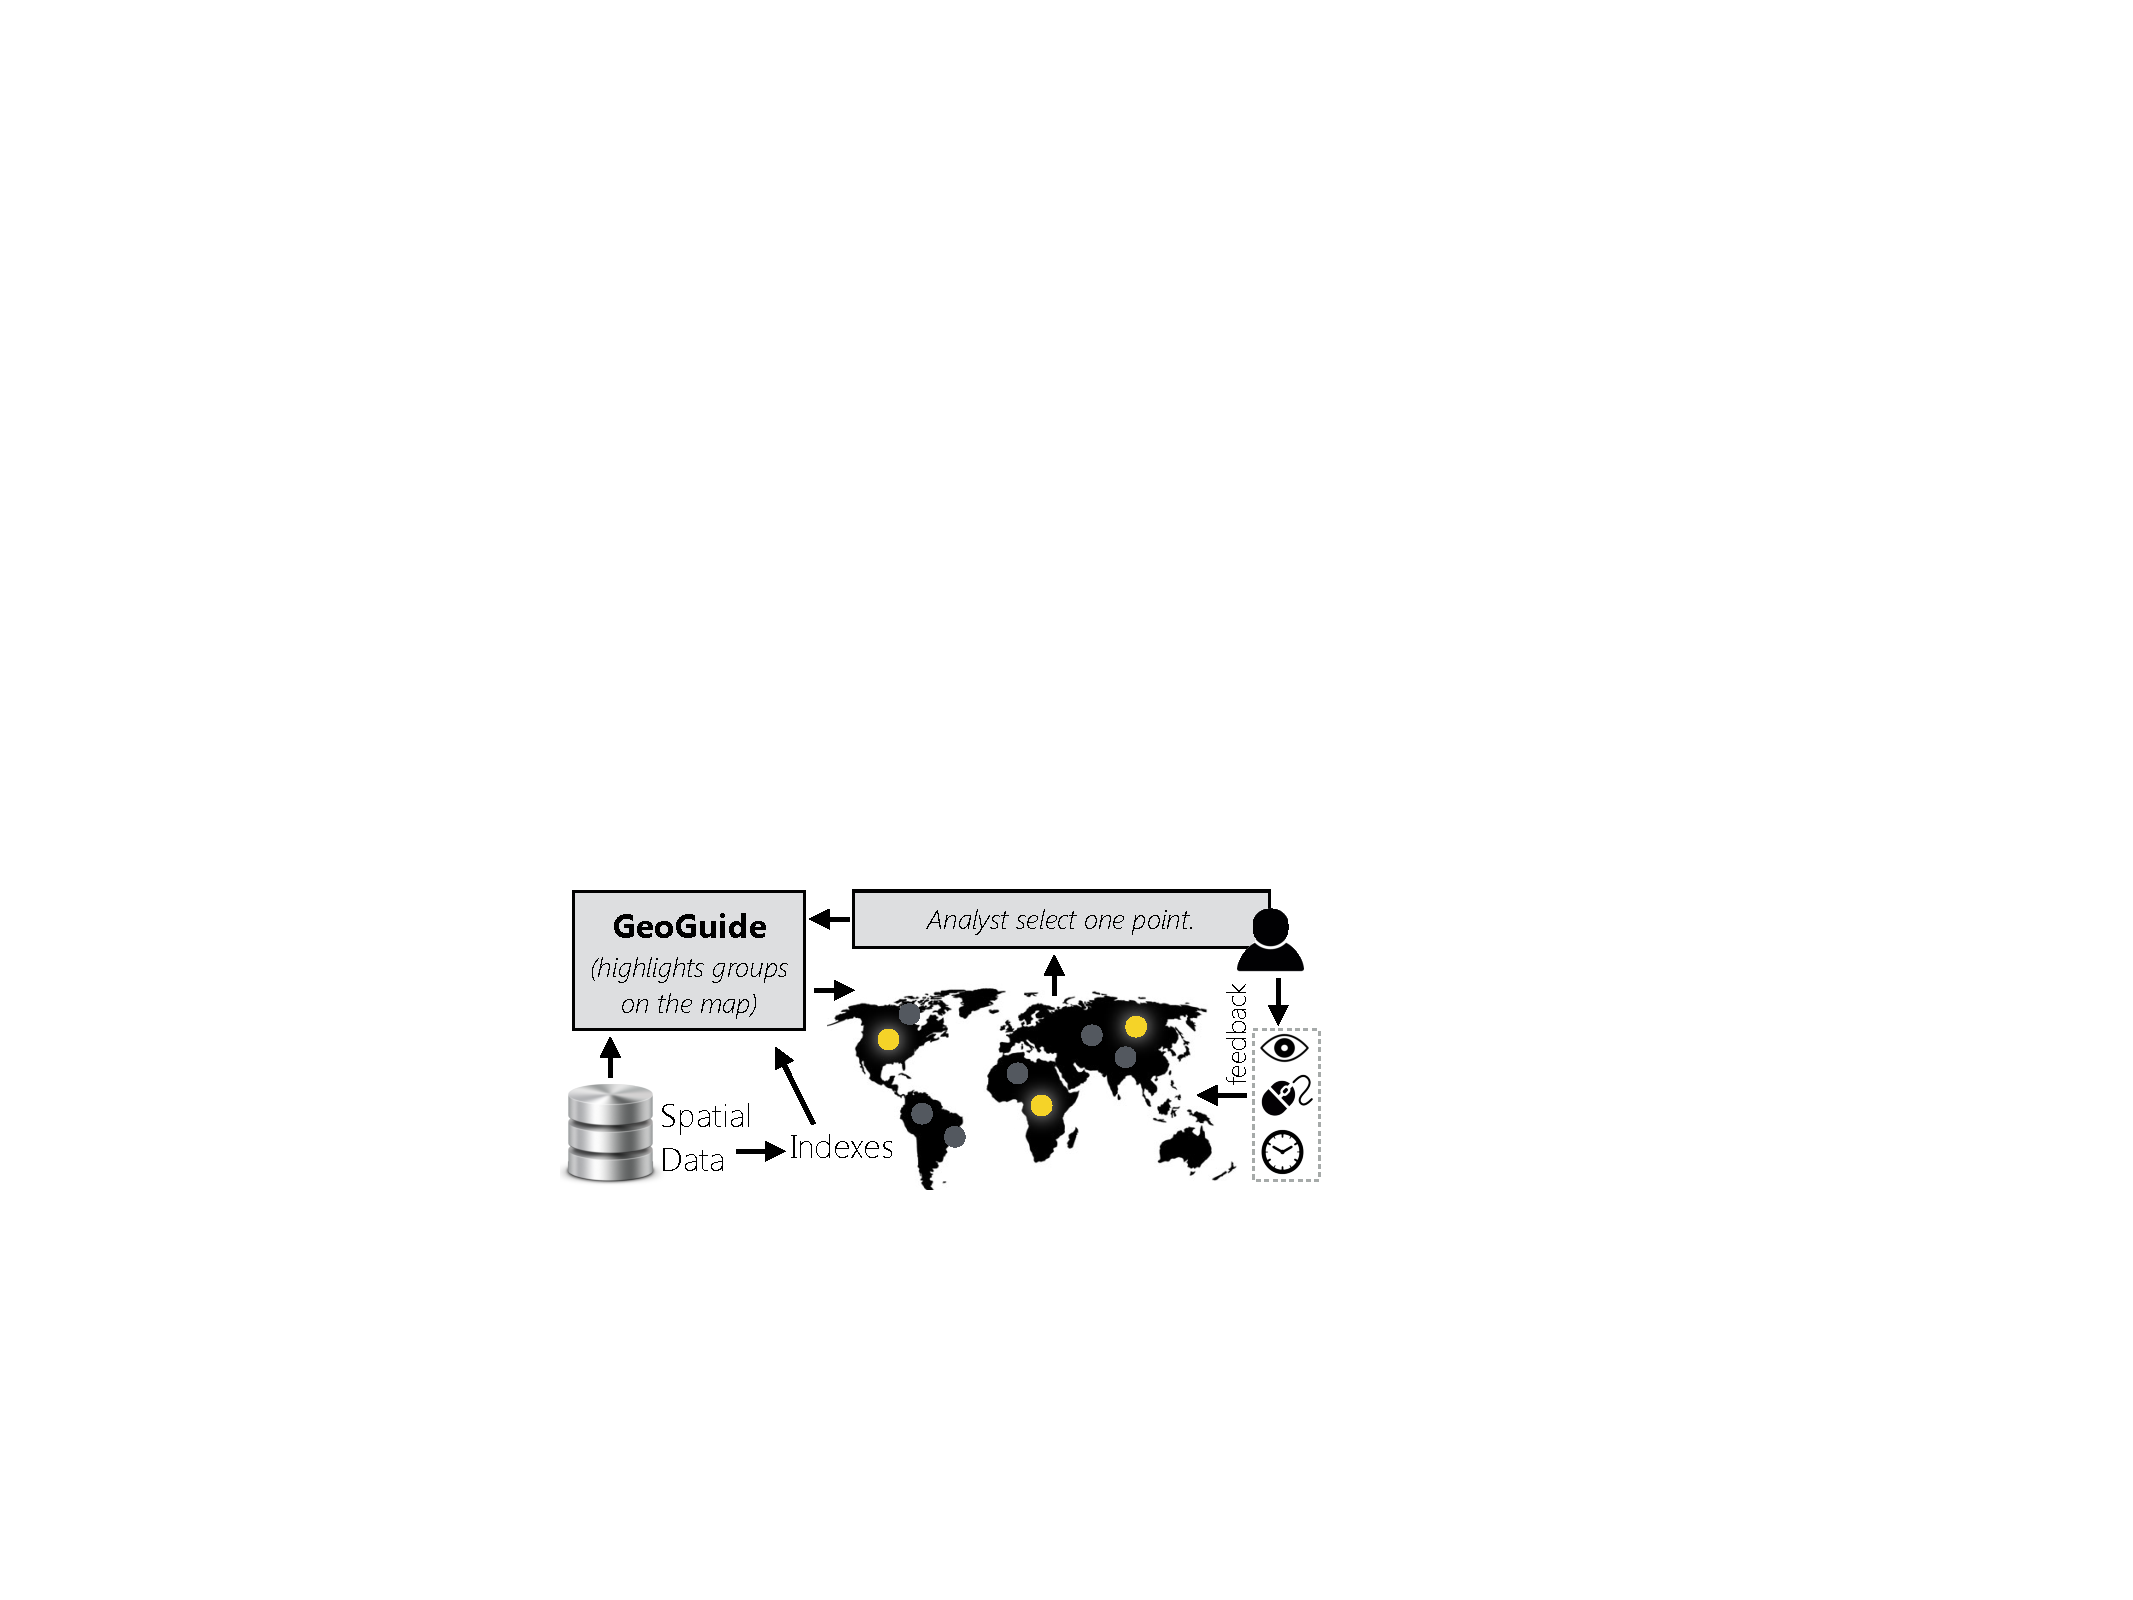
\includegraphics[width=\textwidth]{images/geoguide-pre-processamento.pdf}
	\caption{Visão geral do funcionamento do GeoGuide}
	\label{fig:geoguide-pre-processamento}
	\vspace{-10pt}
\end{figure*}

Após o processamento dessas métricas, o framework vai normalizar esses valores num intervalo de $0,0$ a $1,0$ e orderná-los em sentido decrescente. Esses valores normalizados são os indíces (ver Figura \ref{fig:geoguide-pre-processamento}) que o GeoGuide utilizará nas sugestões de novos pontos para o analista.

Esse processo é demorado, pois tem a complexidade de $\mathcal{O}(n^{2})$ e isso vira um problema com o aumento do volume desses datasets. Então durante esse cálculo o usuário pode ir navegando pelo seu conjunto de dados e ir conhecendo mais sobre os pontos daquele grupo (gerando \textit{feedback} para a ferramenta, como podemos ver na Figura \ref{fig:geoguide-pre-processamento}). Quando for de seu interesse, o analista pode selecionar um ponto e pedir novas sugestões relacionadas com sua escolha, logo, o GeoGuide irá consultar os indíces resultantes do seu processamento inicial e retornará os pontos mais relevantes com a escolha do usuário. Esse processo pode ser realizado diversas vezes para que o analista sempre possa descobrir o que explorar em seguida.

\section{Criação de IDRs}

No mesmo momento que o servidor da plataforma é disparado para realizar o pré-processamento do dataset para gerar os indíces normalizados das métricas principais do GeoGuide, a aplicação do usuário, quando concluir a plotagem do mapa, começará o processo de rastreamento do movimento do mouse.

Como dito anteriormente, essa coleta dos pontos do mouse usuário navegando a plataforma é importante para a criação dos IDRs e sua utilização nas orientações que o GeoGuide vai propor baseado num ponto escolhido pelo usuário. Essa criação de IDRs obedece os intervalos de $20$ segundos para o processo de clusterização dos pontos, utilizando o algoritmo \textit{k-means} para a criação desses clusters, e também o intervalo definido previamente de que, após $3$ momentos de clusterização, serão selecionados os polígonos resultantes da interseção dos clusters de cada momento e isso resultará nas áreas definidas como IDRs.

Esse processo de construção das IDRs acontece todo o tempo em que o usuário esteja utilizando a plataforma e, a cada geração de IDR, essas regiões serão enviadas para o servidor registrando de qual usuário é essa IDR e qual a seção dele no momento de construção. Com essas informações é então possível ter um histórico das regiões de interesse do usuário e usar esses dados para um outro tipo de análise de preferência do usuário levando em consideração outros fatores.

Todo essa operação mostra a importância das criações das IDRs e também demonstra que as aplicações desses dados podem se expandir, dependendo somente de qual a necessidade que se quer suprir com essas informações.

\section{Detectando Outliers}

Com a construção das IDRs acontecendo durante a utilização do GeoGuide pelo usuário, um outro processo também é executado após cada momento de criação dessas regiões. Com cada região encontrada, nós selecionamos os pontos que estão inseridos em cada região e para cada grupo desse efetuamos uma detecção de outliers nessa região levando em consideração os atributos definidos pelo usuário durante o carregamento desse dataset.

Dessa forma, além de registrar a cada minuto quais são as áreas que o usuário tem mais interesse baseado no seu movimento de mouse, nós também gravamos quais são os pontos considerados discrepantes de cada região dessa e, com isso, temos os dados suficientes para o processo final das orientações que o GeoGuide performará quando requerido pelo usuário.

\section{Processamento final}

Desde o momento que o usuário é imerso no mapa global com os pontos de seus datasets plotados, as ações que acontecem são desconhecidas pelo usuário e acontecem sem sua menor interferência ou sem ele conseguir notar seu processamento.

Porém, o momento mais importante para o usuário e que é finalidade de todo esse processo executado em \textit{background}, é quando ele seleciona um ponto de seu interesse e então pede $k$ novos pontos como sugestões do GeoGuide baseado nos atributos do ponto escolhido pelo usuário. Nesse momento é que será levado em consideração as IDRs registradas na sua seção e os outliers detectados em cada região.

Agora, nessa nova proposta do GeoGuide, os pontos que se encontrarem dentro das regiões definidas como IDRs pelo usuário serão priorizados para serem sugeridos, pois assim o usuário conseguirá obter mais informações dentro de uma região que já é previamente definida como interessante para ele e não irá perder seu foco em outras possíveis regiões.

E também, no momento em que o GeoGuide propõe novos pontos para serem analisados, os pontos registrados como outliers dentro das IDRs também serão privilegiados nessa proposta do GeoGuide, pois, como visto em outra pesquisa \cite{DBLP:journals/debu/FreireCVZ16}, esses pontos ``aberrantes'' podem indicar novas características desse dataset e um começo de por onde procurar particularidades desse dataset escolhido pelo usuário.
